\documentclass[conference]{IEEEtran}
\IEEEoverridecommandlockouts

\usepackage[T1]{fontenc}
\usepackage{amsmath,amssymb}
\usepackage{booktabs}
\usepackage{array}
\usepackage{graphicx}
\usepackage{tikz}
\usetikzlibrary{positioning,arrows.meta}
\usepackage{url}
\usepackage[hidelinks]{hyperref}
\hypersetup{
  pdftitle={TorShield: A Transparent In-Kernel Authenticated Tunnel with Fail-Closed TC Steering},
  pdfauthor={Roshan Srikanth and Dr. S. UdhayaKumar},
  pdfkeywords={Linux kernel, network security, authenticated encryption, ChaCha20-Poly1305, Netfilter, eBPF, traffic control}
}

\newcommand{\sys}{\textsc{TorShield}}
\newcommand{\code}[1]{\texttt{#1}}

\title{\sys: A Transparent In-Kernel Authenticated Tunnel with Fail-Closed TC Steering}

\author{
\IEEEauthorblockN{Roshan Srikanth}
\IEEEauthorblockA{Amrita Vishwa Vidyapeetham\\
Email: roshansrikanth21@gmail.com}
\and
\IEEEauthorblockN{Dr. S. UdhayaKumar}
\IEEEauthorblockA{Amrita Vishwa Vidyapeetham\\
Email: sudhayakumar@ch.amrita.edu}
}

\begin{document}
\maketitle

\begin{abstract}
Application-level encryption protects payloads but leaves metadata visible and requires per-application changes. \sys{} is a Linux kernel module that transparently encrypts peer-destined IPv4/IPv6 traffic in UDP using ChaCha20--Poly1305, a 16-byte authenticated header, per-peer 64-bit sequence numbers, a 1024-packet replay window, and 64-byte padding. The same wire format is used by Netfilter, a route-based L3 device, and TC clsact/eBPF steering. For TC, a kernel guard at \code{LOCAL\_OUT}/\code{FORWARD} drops peer-destined packets when the egress classifier or qdisc is removed. We report captured results: 1\,MB IPv4 and 256\,KB IPv6 TCP transfers were byte-exact; independent AEAD verification accepted 1054/1054 tunnel frames; deletion tests blocked 8/8 local sends and 8/8 forwarded packets with zero outer packets; a 30\,s four-stream native VM run sustained 3.40\,Gbit/s with flat unreclaimable memory. We also report four defects found and fixed. \sys{} is not Tor, provides no anonymity, and does not replace WireGuard or IPsec.
\end{abstract}

\begin{IEEEkeywords}
Linux kernel, network security, authenticated encryption, ChaCha20--Poly1305, Netfilter, eBPF, traffic control, replay protection.
\end{IEEEkeywords}

\section{Introduction}

Network operators increasingly classify, throttle, and block traffic using addresses, ports, flow statistics, packet sizes, and timing. Transport Layer Security (TLS) protects content, but it does not hide the metadata that surrounds a connection, and it requires each application to use it. A kernel-level mechanism can apply a uniform policy to every socket without changing applications, which is useful for legacy software, testbeds, and controlled deployments.

This paper describes the current \sys{} design. An earlier draft of this work described a single-byte XOR transform. We explicitly withdraw those claims. A single-byte XOR is trivially recoverable from known plaintext, is length-preserving, and provides no integrity; rotating the byte does not repair those properties. The XOR prototype is retained only as a historical baseline. The system evaluated here is a different datapath: an authenticated UDP tunnel with per-peer keys and a replay window.

\sys{} is deliberately narrow. It is \emph{not} Tor and provides no anonymity, onion routing, or censorship circumvention. It does not disguise protocol signatures, shape timing, or hide outer addresses and ports. It is also not a replacement for WireGuard or IPsec: it has no handshake and no forward secrecy, and its control plane is a set of procfs files. The contribution is an engineering and measurement study of transparent in-kernel tunneling and of a fail-closed TC steering path that is difficult to obtain when Netfilter and TC execute at different points in the stack.

\subsection{Contributions}
\begin{itemize}
\item A kernel datapath and wire format for transparent peer-destined IPv4/IPv6 traffic: ChaCha20--Poly1305, a 32-bit key identifier, 64-bit per-peer sequence numbers, 64-byte padding, a 1024-packet replay window, and per-peer allowed prefixes with authenticated roaming.
\item One wire format shared by Netfilter, a route-based L3 device, and TC clsact/eBPF steering, plus a kernel-side fail-closed TC guard at \code{LOCAL\_OUT}/\code{FORWARD} and loader map completeness. We test classifier and qdisc deletion on local and forwarded paths.
\item An empirical study on two kernel versions and a native VM, with independent AEAD verification, deletion tests, manual rekey, a rate limiter, and a 30\,s sustained run. We report four defects found and fixed, and we withdraw the draft's unverified CPU, latency, footprint, stability, and distribution claims.
\end{itemize}

\section{Threat Model and Scope}

\paragraph{Assets}
The confidential payload is the inner IP packet: its addresses, transport headers, and application data. The outer IP/UDP headers (including TTL and DSCP), the \code{TS} magic, the key identifier, the sequence number, ciphertext length, direction, timing, and approximate size bucket remain visible.

\paragraph{Adversary}
We consider (i) a passive on-path observer that records and classifies packets; (ii) an active off-path sender that injects, replays, or mutates outer datagrams; and (iii) an unprivileged local process that can create sockets but cannot read kernel memory or configure the module. We do not defend against a compromised endpoint, a root attacker who can read keys or modify the kernel, or an adversary who can observe both endpoints.

\paragraph{Assumptions}
The kernel and the module are trusted. Each peer has a 256-bit key configured out of band. Root configures the peer table, mode, and (for TC) the loader. The classifier is attached before the mode is switched to \code{tc}.

\paragraph{Non-goals}
\sys{} provides confidentiality, integrity, and replay resistance for tunneled packets. It does not provide anonymity, traffic-analysis resistance, protocol obfuscation, forward secrecy, automatic key agreement, per-network-namespace policy, or a general denial-of-service defense. Stream mode is legacy, length-preserving, and unauthenticated; it is excluded from the security claims.

\section{Related Work}

\paragraph{Anonymity and censorship resistance}
Tor provides layered encryption and onion routing through relays \cite{dingledine2004tor}. Pluggable transports such as obfs4 and ScrambleSuit modify the observable protocol shape \cite{obfs4,winter2013scramblesuit}, and format-transforming encryption maps ciphertext to a target format \cite{dyer2013fte}. These systems target a different problem: hiding the fact that a flow is Tor or making it resemble another protocol. \sys{} does not attempt either. Work on traffic morphing changes packet sizes and timing \cite{wright2009morphing}, and measurement studies show that naive obfuscation can be fingerprinted \cite{houmansadr2013parrot}. Those results motivate our explicit non-goal: padding to 64-byte buckets reduces exact-length leakage but does not make the traffic unobservable.

\paragraph{Network-layer protection}
IPsec provides authenticated and encrypted IP traffic with a standards-based policy and key-exchange framework \cite{kent2005ipsec}. WireGuard is a compact kernel UDP tunnel with a Noise-based handshake, cryptokey routing, and forward secrecy \cite{donenfeld2017wireguard}. OpenVPN is a userspace TLS-based tunnel. \sys{} shares the UDP/AEAD idea with WireGuard but differs in deployment and scope: it exposes transparent Netfilter steering and a TC/eBPF steering path, uses manually configured per-peer keys, and has no handshake. We do not claim better security or performance than WireGuard; for production privacy, WireGuard or IPsec is the appropriate choice.

\paragraph{Programmable packet processing}
eBPF and TC allow packet classification and redirection in the kernel \cite{hoiland2018xdp}. \sys{} uses a clsact egress classifier only for steering; the AEAD remains in the device's \code{ndo\_start\_xmit} because the BPF helper set cannot call the synchronous in-kernel ChaCha20/Poly1305 path. The fail-closed guard is a separate Netfilter hook, which creates the ordering problem analyzed in Section~\ref{sec:tc}.

\section{System Design}
\label{sec:design}

\subsection{Overview and Modes}
\sys{} is a loadable kernel module. It is inert until a key and at least one peer are configured, so loading it does not disrupt a host. Fig.~\ref{fig:datapath} shows the shared datapath, and Table~\ref{tab:modes} lists the four modes. The default is \code{tunnel}. \code{hybrid} and \code{tc} add alternative egress-steering mechanisms but keep the same wire format and the same Netfilter ingress decapsulation. \code{stream} is the legacy length-preserving transform and is not recommended.

\begin{figure}[t]
\centering
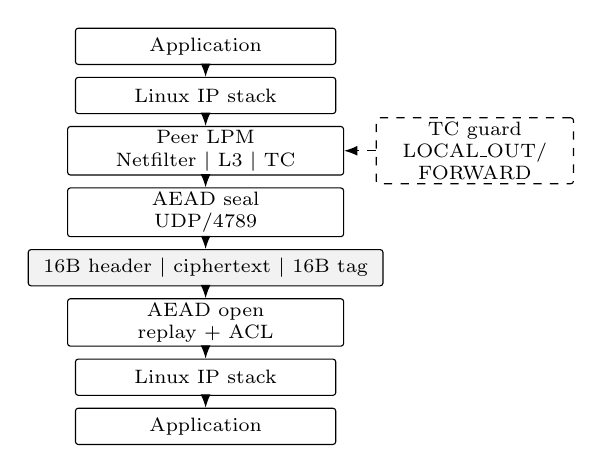
\begin{tikzpicture}[font=\scriptsize,>=Latex,node distance=1.5mm,
  box/.style={draw,rounded corners=1pt,align=center,inner sep=1.5pt,
              minimum height=4.6mm,text width=32mm},
  wire/.style={box,fill=black!5,text width=44mm}]
\node[box] (app) {Application};
\node[box,below=of app] (stack) {Linux IP stack};
\node[box,below=of stack,text width=34mm] (egress) {Peer LPM\\ Netfilter $|$ L3 $|$ TC};
\node[box,below=of egress,text width=34mm] (seal) {AEAD seal\\UDP/4789};
\node[wire,below=of seal] (wire) {16B header $|$ ciphertext $|$ 16B tag};
\node[box,below=of wire,text width=34mm] (open) {AEAD open\\replay + ACL};
\node[box,below=of open] (rstack) {Linux IP stack};
\node[box,below=of rstack] (rapp) {Application};
\node[box,right=4mm of egress,text width=24mm,dashed] (guard) {TC guard\\LOCAL\_OUT/\\FORWARD};
\draw[->,dashed] (guard) -- (egress);
\foreach \a/\b in {app/stack,stack/egress,egress/seal,seal/wire,wire/open,open/rstack,rstack/rapp}
  \draw[->] (\a) -- (\b);
\end{tikzpicture}
\caption{TorShield v4 datapath. All egress modes share one AEAD wire format; the TC guard drops peer-destined packets when the classifier or qdisc is missing.}
\label{fig:datapath}
\end{figure}

\begin{table}[t]
\centering
\caption{Datapath modes. Tunnel, hybrid, and TC share one wire format.}
\label{tab:modes}
\footnotesize
\setlength{\tabcolsep}{3pt}
\begin{tabular}{@{}p{0.15\columnwidth}p{0.77\columnwidth}@{}}
\toprule
Mode & Egress behaviour \\
\midrule
\code{tunnel} & Netfilter \code{POST\_ROUTING} matches the inner destination against peer prefixes, encapsulates, and returns \code{NF\_STOLEN}. Default. \\
\code{hybrid} & A route into a \code{torshield} L3 netdevice is encapsulated by \code{ndo\_start\_xmit}; other peer traffic still uses Netfilter. \\
\code{tc} & A clsact/eBPF classifier on the underlay redirects matching inner packets to a \code{torshield} device; a Netfilter guard at \code{LOCAL\_OUT}/\code{FORWARD} drops peer packets if the classifier is missing. \\
\code{stream} & Legacy length-preserving payload transform; no authentication. Excluded from security claims. \\
\bottomrule
\end{tabular}
\end{table}

\subsection{Wire Format and AEAD}
An outer packet is
\begin{center}
\footnotesize
\code{outer IP | UDP:4789 | 16-byte header | padded ciphertext | 16-byte tag}.
\end{center}
The 16-byte header is the AEAD associated data. It contains a two-byte \code{TS} magic, a one-byte version, a one-byte flags field (bit~0 indicates an inner IPv6 packet), a 32-bit key identifier (zero selects the legacy global PSK), and a 64-bit big-endian per-peer sequence number. The nonce is the 4-byte XOR fold of the outer source and destination addresses followed by the 8-byte sequence number. The plaintext is the complete inner IP packet, zero-padded to a multiple of 64 bytes; the inner header carries the true length and is parsed only after authentication. The tag is 16 bytes. ChaCha20--Poly1305 follows RFC~8439 \cite{nir2018rfc8439}. The ChaCha20 block function is taken from the in-kernel helper and Poly1305 is implemented in the module; the path is synchronous because the asynchronous crypto API cannot be used from a softirq Netfilter hook.

The outer IPv4 identification field is assigned from a per-packet counter. This matters when a large inner UDP datagram is split into multiple outer IP fragments: a constant zero would make fragments from different datagrams indistinguishable to reassembly. The outer UDP checksum is zero over IPv4, which is legal; integrity is provided by the AEAD tag.

\paragraph{Port choice}
The default outer port is 4789, the IANA VXLAN port. Wireshark and similar tools may heuristically label the outer datagrams as VXLAN. That is a display heuristic: the payload is the \code{TS} header and AEAD ciphertext, not a VXLAN encapsulation. The port can be changed at module load.

\subsection{Peer Table and Cryptokey Routing}
Each peer entry contains a 32-byte key, a deterministic 32-bit key identifier (full FNV-1a of the key, with zero reserved), an outer endpoint, and up to eight allowed inner prefixes. Egress selects the peer by longest-prefix match on the inner destination. Ingress looks up the peer by the wire key identifier (or by outer source for a legacy global-PSK peer), authenticates, and then checks the decrypted inner source against that peer's allowed prefixes. A packet whose inner source is outside the allowed set is dropped and counted. The key identifier is a selector, not an authenticator: an observer can read it, but cannot produce a valid tag without the key. After a packet authenticates, a peer configured with a per-peer key may roam to the new outer source address, so a mobile endpoint can change addresses without a control message.

\subsection{Netfilter Datapath}
\label{sec:netfilter}
The module registers hooks per network namespace with \code{register\_pernet\_subsys}. In tunnel mode, egress runs at \code{NF\_INET\_POST\_ROUTING} with priority \code{NF\_IP\_PRI\_LAST}. It skips outer packets, link-local and loopback sources, and packets already marked by the tunnel. It looks up the peer by inner destination; if there is no peer, the packet continues unchanged. Otherwise it handles GSO by segmenting the super-skb into \code{gso\_size} chunks, assigns each segment its own sequence number, and encapsulates each one. The original skb and each segment are released after they are copied. The hook returns \code{NF\_STOLEN}. On ingress, \code{NF\_INET\_LOCAL\_IN} runs after IP reassembly. It accepts only UDP packets to the configured port; a packet with a non-\code{TS} header is left alone. A framed packet is rate-limited (if enabled), linearized, authenticated, replay-checked after authentication, ACL-checked, and re-injected with \code{netif\_rx}. Any parsing, authentication, replay, ACL, or allocation failure in tunnel mode drops the packet and increments a counter; it is never forwarded as plaintext.

A TCP SYN is clamped to an MSS of 1360 bytes for IPv4 and 1340 bytes for IPv6 so that the outer packet fits in a 1500-byte MTU. Large inner UDP datagrams are allowed to fragment at the outer IP layer; the receiver reassembles and then linearizes before the AEAD. The current implementation verifies 4\,KB and 60\,KB inner datagrams.

\subsection{Hybrid L3 Device}
\code{torshield0} is an \code{ARPHRD\_NONE} L3 netdevice created with \code{ip link add ... type torshield}. It has no L2 header, no ARP, no queueing discipline, an MTU of 1360, and no GSO/TSO offloads. A route such as \code{ip route add 10.0.0.2/32 dev torshield0} sends selected prefixes into \code{ndo\_start\_xmit}, which reuses the same encapsulation functions. The outer route lookup is pinned to the underlay interface supplied as \code{IFLA\_LINK}; this prevents the outer route from matching the route into the device and recursing. In hybrid mode the Netfilter egress hook skips packets whose route already points at a \code{torshield} device, while all other peer traffic keeps the transparent path. A TC redirect hands the device a full L2 frame, so \code{ndo\_start\_xmit} strips the link header before parsing the inner IP packet.

\subsection{TC Steering and the Fail-Closed Guard}
\label{sec:tc}
TC mode replaces routes with a clsact egress classifier on the underlay. The BPF program \code{ts\_tc\_egress} looks up the inner destination in LPM tries for IPv4 and IPv6, skips multicast and link-local traffic, and redirects a match to the \code{torshield} device ifindex stored in its \code{cfg} map. Outer frames carry mark \code{0x5454} so they are not redirected twice. If a peer matches but \code{cfg[0]} has no redirect target, the program returns \code{TC\_ACT\_SHOT} rather than \code{TC\_ACT\_OK}; a matching packet must never fall through to the wire.

The difficult case is classifier removal. Netfilter \code{POST\_ROUTING} runs before TC egress. In TC mode the Netfilter egress hook is bypassed (otherwise packets would be encapsulated twice), so relying on the classifier alone would be fail-open if the qdisc or program disappeared. \sys{} therefore registers IPv4/IPv6 \code{NF\_INET\_LOCAL\_OUT} and \code{NF\_INET\_FORWARD} hooks at the first priority, both before \code{POST\_ROUTING}. For a peer-destined packet, the guard uses \code{nf\_hook\_state.out} (not \code{skb\_dst}, which can still describe the input route at \code{FORWARD}) and accepts only if:
\begin{enumerate}
\item the output device is a \code{torshield} device, which encapsulates in \code{ndo\_start\_xmit}; or
\item the output device still has a live TC egress classifier---a TCX program named \code{ts\_tc\_egress} in \code{dev->tcx\_egress}, or a live \code{cls\_bpf} filter in the clsact mini-Qdisc (the style the loader uses today).
\end{enumerate}
Otherwise the guard returns \code{NF\_DROP} and increments \code{tc\_guard}. A local \code{sendto()} then fails with \code{EPERM}; no clear frame reaches the underlay. The TCX branch is compile-tested only; the runtime tests use the clsact path.

The guard proves only that a classifier is attached; it does not prove that the classifier's maps are complete. \code{torshield-tc attach} reads every \code{allowed=} prefix from \code{/proc/torshield/peers} and fills the LPM tries before switching the mode to \code{tc}. If a peer is added, deleted, or cleared while the mode is \code{tc}, the kernel forces the mode back to \code{tunnel} until the loader reruns. Direct map edits or a hand-loaded classifier are outside the guarantee. The loader and the peer-list update are not one atomic transaction, so operators must not reconfigure peers concurrently with \code{attach}.

\paragraph{Residual race}
The guard and the later TC egress hook read the attachment separately. If a classifier is deleted after the guard accepts a packet but before that packet reaches egress, that one in-flight packet can still leave in clear. The deletion tests in Section~\ref{sec:eval} prove fail-closed behaviour for all subsequent packets, not a zero-race guarantee. Closing this requires a last-chance \code{ndo\_start\_xmit} check or a single authoritative steering point; neither is implemented.

\subsection{Replay, Rate Limiting, and Manual Rekey}
The receiver keeps a 1024-packet sliding window per peer. A sequence of zero is invalid. The window is advanced only after successful authentication, so an off-path packet cannot consume a window slot. The window was widened from 64 packets after four-stream native traffic produced 229 false replay drops; with 1024 packets the same run produced zero.

An optional per-source fixed-window limiter (\code{ts\_rl\_pps}, default zero) runs before \code{skb\_linearize} and Poly1305. It bounds the crypto work a single source can force, but it is not a cookie challenge and the source address is spoofable. It is disabled by default so that measurements are not capped.

Per-peer keys can be rotated manually. \code{rekey-peer} moves the current key to a previous slot and starts sending with the new key; the receiver accepts both key identifiers until \code{rekey-commit} erases the previous key. A second rotation before commit is rejected, so the oldest key cannot be silently discarded. This protects packets already in flight, but both ends must be reconfigured and traffic can drop between the two commands. There is no handshake and no forward secrecy.

\section{Implementation}
The canonical module is \code{module/LKM/torshield.c}; the TC classifier and loader are in \code{module/LKM/tc/}. The control plane is \code{/proc/torshield/\{psk,peers,mode,stats\}} with a thin \code{torshieldctl} wrapper. The peer file accepts \code{+endpoint key HEX allowed PREFIX,...} and \code{-endpoint} / \code{clear}; the stats file exposes tunnel, device, ACL, roaming, rate-limit, and guard counters. The module registers ten hooks per network namespace: six datapath hooks (IPv4/IPv6 \code{PRE\_ROUTING}, \code{POST\_ROUTING}, \code{LOCAL\_IN}) and four guard hooks (IPv4/IPv6 \code{LOCAL\_OUT}, \code{FORWARD}).

The TC loader is a libbpf program. It loads \code{torshield\_tc.o}, fills the LPM and \code{cfg} maps, attaches the program to the underlay's clsact egress, and only then writes \code{tc} to the mode file. \code{detach} writes \code{tunnel} first and then removes the qdisc. A watchdog can poll the attachment and revert the mode, but it is a recovery aid, not the security boundary.

The module builds cleanly with \code{make W=1} against Ubuntu 24.04 kernels 6.8.0-147 and 6.17.0-42, and against the native 6.18.54.1 headers used for the performance runs. The 6.16 ChaCha API change (opaque state array to \code{struct chacha\_state}) is handled with a version-conditional shim. The TC object and loader build with \code{-Wall -Wextra} clean.

\section{Evaluation}
\label{sec:eval}

\subsection{Methodology and Environment}
Correctness, deletion, and interoperability tests run in an Ubuntu 24.04 QEMU 8.2 guest with kernel 6.8.0-147 and TCG (no KVM). The guest uses network namespaces \code{n1}/\code{n2} connected by a veth pair; a third namespace \code{n3} is used for the forwarded-path test. Throughput is measured separately on the native WSL2 kernel 6.18.54.1 (Hyper-V, 16 vCPUs), because TCG CPU emulation is not a throughput measurement. The native host is a VM, not bare metal. The direct-veth baseline is about 100\,Gbit/s, so the link is not the bottleneck; the tunnel is CPU-bound.

Each run starts from a clean module, configures keys and peers, and captures outer packets. A host-side Python verifier independently reconstructs the nonce and AAD and decrypts each frame with the \code{cryptography} package. Counters are read from \code{/proc/torshield/stats}. The test harness and per-stage scripts are part of the artifact.

\subsection{Correctness and Interoperability}
Table~\ref{tab:correctness} summarizes the functional results. The IPv4 TCP transfer was byte-exact, the IPv6 transfer was byte-exact, and the independent verifier accepted every captured frame. The large-UDP cases exercise outer fragmentation and reassembly. Replay, tamper, and unknown-source packets were dropped with exact counter increments. TC and hybrid paths used distinct inner and outer prefixes, so a successful transfer also demonstrates cryptokey routing rather than address coincidence.

\begin{table}[t]
\centering
\caption{Verified correctness and interoperability results. All values are from captured runs, not projections.}
\label{tab:correctness}
\footnotesize
\setlength{\tabcolsep}{3pt}
\begin{tabular}{@{}p{0.49\columnwidth}p{0.43\columnwidth}@{}}
\toprule
Test & Result \\
\midrule
Tunnel, IPv4 TCP 1\,MB & 1\,048\,576/1\,048\,576 bytes (100\%) \\
Tunnel, IPv6 TCP 256\,KB & 262\,144/262\,144 bytes (100\%) \\
Independent AEAD, tunnel capture & 1054/1054 frames accepted \\
Tunnel, 4\,KB inner UDP & 4000/4000 bytes; 3 outer fragments \\
Tunnel, 60\,KB inner UDP & 60000/60000 bytes; 41 outer fragments \\
Replay / tamper / unknown peer & each dropped; counters exact \\
Hybrid, IPv4 TCP 1\,MB & 100\%; 807/807 frames accepted \\
Hybrid, IPv6 TCP 256\,KB & 100\%; 209/209 frames accepted \\
Cryptokey routing, v4/v6 echo & 256/256 and 64/64 \\
TC, IPv4 UDP echo & 256/256; \code{dev\_out} 512; \code{tun\_out} 0 \\
TC, IPv6 UDP echo & 64/64; \code{dev\_out} 647 (cumulative); \code{tun\_out} 0 \\
TC detach fallback & mode \code{tunnel}; echo 16/16 \\
\bottomrule
\end{tabular}
\end{table}

\subsection{Wire-Format Verification}
Independent AEAD verification accepted 1054/1054 tunnel frames, 807/807 hybrid IPv4 frames, 209/209 hybrid IPv6 frames, 210/210 TC IPv4 frames, and 68/68 TC IPv6 frames with the correct key. The TC captures accepted 0/210 and 0/68 when verified with the global PSK, confirming that key selection is actually in use. The native IPv6 pcap capture was empty in the WSL2 harness, so the IPv6 wire claim rests on the QEMU 68/68 capture; native IPv6 was verified functionally by echo and counters.

\subsection{TC Fail-Closed Behaviour}
Table~\ref{tab:guard} reports the deletion tests. In the \code{LOCAL\_OUT} test, a local socket sends eight packets while the classifier is deleted; all eight fail with \code{EPERM}, the peer server receives zero, \code{tc\_guard} increases by eight, and both \code{dev\_out} and \code{tun\_out} remain unchanged. Deleting the clsact qdisc produces the same result. Reattaching the classifier restores a 16/16 echo; detaching falls back to the Netfilter path at 8/8.

The \code{FORWARD} test injects raw frames on \code{n1}, so the sender's \code{LOCAL\_OUT} hook is bypassed. With no classifier, \code{n2} receives eight forwarded inner packets, \code{n3} sees zero outer packets, \code{tc\_guard} increases by eight, and \code{dev\_out} does not move. With the classifier present, \code{tc\_guard} stays flat, \code{dev\_out} increases by eight, and \code{n3} records eight \code{tun\_rx}. Deleting the classifier returns to zero outer packets and a guard increase of eight. This is the empirical basis for the fail-closed claim, with the residual race noted in Section~\ref{sec:tc}.

\begin{table}[t]
\centering
\caption{TC fail-closed tests. Values are deltas over the test window.}
\label{tab:guard}
\footnotesize
\setlength{\tabcolsep}{2.5pt}
\begin{tabular}{@{}p{0.38\columnwidth}p{0.57\columnwidth}@{}}
\toprule
Condition & Observed result \\
\midrule
\code{LOCAL\_OUT}, classifier deleted & 0 sent / 8 blocked (\code{EPERM}); server 0; \code{tc\_guard} +8; \code{dev\_out} +0; \code{tun\_out} +0 \\
\code{LOCAL\_OUT}, qdisc deleted & same: 0/8; server 0; \code{tc\_guard} +8; \code{dev\_out} +0; \code{tun\_out} +0 \\
\code{LOCAL\_OUT}, classifier restored & echo 16/16; detach fallback 8/8 \\
\code{FORWARD}, no classifier & \code{n2} ingress 8; \code{n3} outer 0; \code{tc\_guard} +8; \code{dev\_out} +0 \\
\code{FORWARD}, classifier present & \code{tc\_guard} +0; \code{dev\_out} +8; \code{n3} \code{tun\_rx} +8 \\
\code{FORWARD}, classifier deleted & \code{n3} outer 0; \code{tc\_guard} +8; \code{dev\_out} +0 \\
Peer add/del/clear in \code{tc} & each forces mode \code{tunnel} \\
Loader auto-fill, no \code{-4/-6} & 2 IPv4 + 2 IPv6 prefixes; echo 16/16 \\
\bottomrule
\end{tabular}
\end{table}

\subsection{Manual Rekey and Rate Limiting}
On the native kernel, a rekey changed the egress key identifier from 4290739141 to 1666914373. During the grace period, four payloads using the old and new keys were all accepted. After \code{rekey-commit}, one old-key packet was rejected as non-peer traffic: \code{tun\_in} increased by four, \code{tun\_peer} by one, and \code{tun\_replay} stayed zero. A same-key no-op returned success; a second rotation before commit, a commit without a previous key, and invalid hex all returned errors without changing state.

With \code{ts\_rl\_pps=50}, 950 of 1000 synthetic packets were rejected before the AEAD and 50 reached it; a legitimate 64-packet echo still completed 64/64. This demonstrates the limiter's placement, not a general DoS defense.

\subsection{Performance}
Table~\ref{tab:perf} reports the native VM measurements. The baseline is direct veth with four TCP streams. The tunnel is CPU-bound: one stream reaches about 0.91--0.97\,Gbit/s and four streams reach 3.02--3.35\,Gbit/s. A separate 30\,s four-stream run sustained 3.40\,Gbit/s with zero tunnel drops and zero replays; \code{SUnreclaim} stayed flat at 63--68\,MB. A 100-ping RTT run averaged 0.052\,ms through the tunnel; this is a VM measurement, not a tail-latency study, and we do not report the draft's 0.5\,ms per-packet figure.

\begin{table}[t]
\centering
\caption{Native WSL2/Hyper-V measurements (kernel 6.18.54.1, 16 vCPUs). Not bare metal.}
\label{tab:perf}
\footnotesize
\setlength{\tabcolsep}{3pt}
\begin{tabular}{@{}p{0.50\columnwidth}p{0.42\columnwidth}@{}}
\toprule
Test & Result \\
\midrule
Baseline, direct veth, 4 streams & 100.98 / 99.76 / 97.84\,Gbit/s \\
Tunnel, 1 stream & 909.7 / 921.5 / 965.4\,Mbit/s \\
Tunnel, 4 streams & 3345.6 / 3018.1 / 3203.1\,Mbit/s \\
Tunnel, 30\,s sustained, 4 streams & 3.40\,Gbit/s; \code{tun\_drop} 0; \code{tun\_replay} 0 \\
Unreclaimable slab, 30\,s run & flat at 63--68\,MB \\
Tunnel RTT, 100 pings & 0.052\,ms average \\
\bottomrule
\end{tabular}
\end{table}

\subsection{Defects Found and Fixed}
The evaluation exposed four defects that static review did not. Table~\ref{tab:defects} lists them. The GSO leak is the most serious: the egress loop copied each segment into an outer skb but did not release the original segment, so a 30\,s four-stream run drove unreclaimable slab to about 7.4\,GB and panicked the VM. The replay window was too small for parallel-queue reordering. The receive path read a reassembled fragmented skb through a linear pointer. The outer IPv4 ID was always zero. All four are fixed in the current code and covered by the regression runs.

\begin{table}[t]
\centering
\caption{Defects exposed by the evaluation and fixed in the current code.}
\label{tab:defects}
\footnotesize
\setlength{\tabcolsep}{2.5pt}
\begin{tabular}{@{}p{0.30\columnwidth}p{0.66\columnwidth}@{}}
\toprule
Defect & Evidence and fix \\
\midrule
GSO skb leak & 30\,s four-stream run drove \code{SUnreclaim} to about 7.4\,GB and panicked; \code{consume\_skb(seg)} after encapsulation; same run flat at 63--68\,MB. \\
Replay window too small & 64-packet window produced 229 false replay drops and 107 retransmits on four streams; 1024-packet window produced zero replays. \\
Fragmented-skb read & Reassembled outer datagrams failed AEAD because the ciphertext was read only from the linear head; \code{skb\_linearize()} before the AEAD. \\
Outer IPv4 ID zero & All outer datagrams carried ID 0; per-packet counter and IPv4 checksum fix. \\
\bottomrule
\end{tabular}
\end{table}

\subsection{Withdrawn Claims}
The initial draft reported 1\% additional CPU, 0.5\,ms per packet, a 50\,KB kernel footprint, 5\% throughput loss, 72-hour stability, and a matrix of Ubuntu, CentOS, and Debian kernels. Those numbers are not reproduced by the current system and are not used here. In particular, we did not measure CPU utilization or per-packet processing time; the module-size and long-duration stability claims are not part of this study; and the build matrix in this paper is Ubuntu 24.04 with kernels 6.8.0-147 and 6.17.0-42 plus the native 6.18.54.1 VM.

\subsection{Threats to Validity}
The throughput numbers come from a WSL2/Hyper-V VM, not bare metal, and from veth rather than a physical NIC. Checksum and offload behavior on a real NIC is not validated. The TC deletion tests are IPv4 only; the IPv6 guard hooks build but are not separately tested for removal. The TCX branch is compile-tested only. The rekey test is IPv4 only. The native IPv6 pcap capture is empty in this harness, so the IPv6 wire evidence is the QEMU capture. The performance suite does not isolate CPU time per packet, and the RTT run is short. These limitations bound the claims; they do not affect the byte-exact correctness or the deletion counters.

\section{Security Analysis}

\paragraph{Protections}
The AEAD provides confidentiality and integrity for the inner IP packet, including its addresses and transport headers. The 64-bit per-peer sequence number and the 1024-packet window reject replays after authentication. The key identifier selects a per-peer key; the inner source ACL prevents a peer from injecting a source prefix it does not own. Endpoint roaming occurs only after authentication, so an off-path attacker cannot redirect a peer by spoofing an outer source. In tunnel and hybrid modes, all authentication and parsing failures drop the packet. In TC mode, the guard drops peer-destined packets when the classifier is missing, and the classifier itself drops a matching packet when its redirect target is unset. Padding to 64-byte buckets reduces exact-length leakage.

\paragraph{Residual risks}
Outer addresses, ports, the \code{TS} magic, key identifier, sequence number, ciphertext length, direction, timing, and approximate size bucket are visible. The system does not resist traffic analysis or DPI. There is no handshake, no forward secrecy, and no automatic key agreement; a compromised key exposes the traffic it protects, and a compromised endpoint exposes plaintext. The peer table, key, and mode are global across network namespaces. The rate limiter is a fixed-window filter, not a cookie challenge, and the source is spoofable. The TC guard has a narrow check-to-egress race; the deletion tests prove fail-closed behavior for subsequent packets, not absolute zero-race closure. The TCX path is not runtime-tested. TC and hybrid mode are prototypes, not production-hardened transports. The legacy stream mode has no integrity and is excluded.

\paragraph{Not Tor}
\sys{} does not provide anonymity. It does not use onion routing, cover traffic, or a distributed relay network. Its name is historical. A user who needs anonymity should use Tor; a user who needs a production VPN should use WireGuard or IPsec.

\section{Discussion and Lessons}
Three lessons recur. First, transparency is not free: the same packet can be selected by Netfilter, a route, or TC, and the ordering of those mechanisms determines both correctness and failure behavior. The TC guard exists because \code{POST\_ROUTING} runs before TC egress; a fail-closed design needs a check before the point where the packet can escape. Second, GSO and skb ownership are the main kernel pitfalls. The byte-exact tests passed while the GSO path leaked memory, and only a sustained run exposed it. Third, replay-window sizing is a property of the deployment's parallelism, not a constant: a 64-packet window was adequate for a single stream and wrong for four streams on parallel queues.

The negative result about the XOR prototype is also a lesson. A length-preserving transform can be described as ``obfuscation'' and still be trivially invertible; without authentication and a nonce discipline, it is not a security mechanism. Replacing it with an AEAD forced a different framing, a sequence number, a replay window, and a key identifier---and made the evaluation meaningful.

\section{Conclusion and Future Work}
\sys{} is a transparent in-kernel authenticated tunnel with three steering paths and a kernel-side fail-closed guard for TC. The current code is byte-exact on IPv4 and IPv6 TCP, survives independent AEAD verification, drops replay/tamper/unknown-source packets, and blocks subsequent local and forwarded packets when the TC classifier is removed. On a native VM it sustains 3.40\,Gbit/s over four streams for 30\,s with flat unreclaimable memory. The paper also reports the defects that the evaluation found and the claims that the earlier XOR draft cannot support.

Future work is concrete: close the guard-to-egress race with a last-chance transmit check or a single steering point; add a handshake and forward secrecy; move the control plane to netlink and make state per-network-namespace; deliver decapsulated packets through the tunnel device so policy routing and \code{rp\_filter} see them; advertise GSO/TSO on the device and segment in the driver; run the deletion suite for IPv6 and the TCX path; and repeat the throughput study on bare metal with a physical NIC. Until then, \sys{} remains a research and teaching artifact, not a production replacement for WireGuard or IPsec. The code and test harness are available at \url{https://github.com/roshansrikanth21/TorShield}.

\bibliographystyle{IEEEtran}
\bibliography{references}

\end{document}
